%% =====================================================================
%%  CLOUT: Campaigning on a Social Network
%%  Project report, team Dumbocracy
%%
%%  Build:  pdflatex main && bibtex main && pdflatex main && pdflatex main
%%          (or latexmk -pdf main, or upload this folder to Overleaf)
%% =====================================================================
\documentclass[11pt,a4paper,oneside]{report}

%% ---------- Page and fonts ------------------------------------------
\usepackage[a4paper,top=2.6cm,bottom=2.6cm,left=2.5cm,right=2.5cm,headheight=14pt]{geometry}
\usepackage[T1]{fontenc}
\usepackage[utf8]{inputenc}
\usepackage{newpxtext}            % Palatino-like text
\usepackage{newpxmath}            % matching maths (also supplies the AMS symbols)
\usepackage[scaled=0.86]{beramono}% readable monospace for code names
\usepackage{microtype}
\linespread{1.08}

%% ---------- Maths, tables, figures, algorithms -------------------------
\usepackage{mathtools}
\usepackage{booktabs,tabularx,array,multirow}
\usepackage{graphicx}
\usepackage[font=small,labelfont=bf,margin=0.5cm]{caption}
\usepackage{subcaption}
\usepackage{enumitem}
\setlist{itemsep=2pt,topsep=4pt,parsep=0pt}
\usepackage{xcolor}
\usepackage{tikz}
\usetikzlibrary{positioning,arrows.meta,fit,calc,shapes.geometric,backgrounds}
\usepackage{pgfplots}
\pgfplotsset{compat=1.16}
\usepackage{algorithm}
\usepackage[noend]{algpseudocode}
\algrenewcommand\algorithmicrequire{\textbf{Input:}}
\algrenewcommand\algorithmicensure{\textbf{Output:}}
\algrenewcommand\alglinenumber[1]{\footnotesize #1}

%% ---------- Colours ---------------------------------------------------
\definecolor{ink}{HTML}{1F2A44}
\definecolor{accent}{HTML}{2E5E8C}
\definecolor{soft}{HTML}{E8EEF5}
\definecolor{softgreen}{HTML}{E7F2EA}
\definecolor{softsand}{HTML}{F6EFE2}
\definecolor{todo}{HTML}{C0392B}

%% ---------- Headings, headers -----------------------------------------
\usepackage{titlesec}
\titleformat{\chapter}[display]
  {\normalfont\bfseries\color{ink}}
  {\large\scshape\color{accent}Chapter \thechapter}
  {4pt}
  {\Huge}
  [\vspace{2pt}{\color{accent}\titlerule[0.8pt]}]
\titlespacing*{\chapter}{0pt}{-10pt}{22pt}
\titleformat{\section}{\normalfont\Large\bfseries\color{ink}}{\thesection}{0.8em}{}
\titleformat{\subsection}{\normalfont\large\bfseries\color{ink}}{\thesubsection}{0.8em}{}
\titleformat{\subsubsection}{\normalfont\normalsize\bfseries\itshape\color{ink}}{}{0em}{}
\setcounter{secnumdepth}{2}
\setcounter{tocdepth}{1}

\usepackage{fancyhdr}
\pagestyle{fancy}
\fancyhf{}
\fancyhead[L]{\small\color{accent}\nouppercase{\leftmark}}
\fancyhead[R]{\small\color{accent}CLOUT}
\fancyfoot[C]{\small\thepage}
\renewcommand{\headrulewidth}{0.4pt}
\fancypagestyle{plain}{\fancyhf{}\fancyfoot[C]{\small\thepage}\renewcommand{\headrulewidth}{0pt}}

%% ---------- References and links ---------------------------------------
\usepackage[numbers,sort&compress]{natbib}
\usepackage[hidelinks]{hyperref}
\hypersetup{pdftitle={CLOUT: Campaigning on a Social Network},
            pdfauthor={Team Dumbocracy},
            pdfsubject={Multi-Agent Systems course project report}}
\usepackage[nameinlink,capitalise]{cleveref}
\crefname{algorithm}{Algorithm}{Algorithms}
\usepackage{url}
\urlstyle{same}

%% ---------- Macros ----------------------------------------------------
\newcommand{\todo}[1]{\textcolor{todo}{\textbf{[TODO:} #1\textbf{]}}}
\newcommand{\coins}[1]{#1~coins}
\newcommand{\simplex}{\Delta}
\newcommand{\TV}{\operatorname{TV}}
\newcommand{\sig}{\operatorname{sig}}
\newcommand{\E}{\mathbb{E}}
\newcommand{\R}{\mathbb{R}}
\newcommand{\code}[1]{\texttt{#1}}
\newcommand{\ORACLE}{\textsc{Oracle}}
\DeclareMathOperator*{\argmax}{arg\,max}
\DeclareMathOperator*{\argmin}{arg\,min}
\newcommand{\repo}{\url{https://github.com/saikaushhikp/CLOUT}}

\newcommand{\overviewsection}{\section{Overview}}
\newcommand{\summarysection}{\section{Summary}}

%% ---------- TikZ styles -----------------------------------------------
\tikzset{
  box/.style={draw=accent,line width=0.6pt,rounded corners=3pt,fill=soft,
              align=center,inner sep=4pt,font=\small,
              execute at begin node={\hyphenpenalty=10000 \exhyphenpenalty=10000 }},
  boxg/.style={box,fill=softgreen},
  boxs/.style={box,fill=softsand},
  obj/.style={draw=accent,line width=0.6pt,rounded corners=2pt,fill=white,
              align=left,inner sep=3pt,font=\scriptsize,text width=3.9cm,
              execute at begin node={\hyphenpenalty=10000 \exhyphenpenalty=10000 }},
  arr/.style={-{Stealth[length=2.4mm]},line width=0.6pt,color=ink},
  darr/.style={{Stealth[length=2.4mm]}-{Stealth[length=2.4mm]},line width=0.6pt,color=ink},
  msg/.style={-{Stealth[length=2mm]},line width=0.55pt,color=ink},
  ret/.style={-{Stealth[length=2mm]},line width=0.55pt,color=accent,densely dashed},
}

\begin{document}

%% =====================================================================
%%  Title page
%% =====================================================================
\begin{titlepage}
\centering
\vspace*{1.2cm}
{\large\scshape\color{accent} Multi-Agent Systems \textendash{} Course Project Report\par}
\vspace{1.4cm}
{\color{ink}\rule{\linewidth}{0.8pt}\par}
\vspace{0.5cm}
{\fontsize{30}{36}\selectfont\bfseries\color{ink} CLOUT\par}
\vspace{0.35cm}
{\LARGE\color{ink} Campaigning on a Social Network\par}
\vspace{0.4cm}
{\large\itshape Consensus with Logic Optimization in Utility driven Targeting\\
in Multi-agent Election Dynamics\par}
\vspace{0.5cm}
{\color{ink}\rule{\linewidth}{0.8pt}\par}
\vspace{1.2cm}

{\large Team \textbf{Dumbocracy}\par}
\vspace{0.6cm}
\begin{tabular}{ll}
\toprule
\textbf{Name} & \textbf{Roll number} \\
\midrule
Pakki Sai Kaushik            & AI23BTECH11017 \\
G.~Madhava Asrith Murthy     & AI23BTECH11007 \\
Vuppula Hemanth Reddy        & AI23BTECH11033 \\
Vishank Singh                & AI23BTECH11032 \\
B.~U.~Deekshith Patel        & AI23BTECH11003 \\
\bottomrule
\end{tabular}

\vspace{1.4cm}
{\large Under the guidance of \todo{instructor name}\par}
\vspace{0.3cm}
{\large Indian Institute of Technology Hyderabad\par}
\vspace{0.3cm}
{\large November 2026\par}
\vfill
{\small Code repository: \repo\par}
\end{titlepage}

%% =====================================================================
%%  Front matter
%% =====================================================================
\pagenumbering{roman}

\chapter*{Abstract}
\addcontentsline{toc}{chapter}{Abstract}

An election campaign is a contest fought on a network. A party spends money to change what people think,
but people also change each other's minds, and the party never sees the electorate directly. We built
CLOUT, a single-player election game, to study this situation with the tools of multi-agent systems.

The electorate has between ten thousand and one million simulated voters. They live in four regions and
are linked by a friendship network. Each voter wants the government budget split across five sectors in a
particular way. The player writes a manifesto (their own budget split) and then has a few campaign rounds
to win a majority. Each round they may hire party workers, who start word-of-mouth cascades through the
network; buy regional media airings; and pay for survey questions. Meanwhile, every voter drifts towards
the average opinion of their friends.

The game connects several course topics in one place. Opinion drift is DeGroot consensus with stubborn
agents; party workers spread influence by an Independent Cascade; choosing a manifesto is an optimisation
problem on the probability simplex, which we solve with projected gradient and ADMM; and the player's
uncertainty about the electorate is described by epistemic logic, with temporal logic describing how a
campaign unfolds. We implemented the whole model as one PyTorch code path that runs a single world on a CPU
or hundreds of worlds at once on a GPU, together with Bayesian and scripted computer players, a
formal-reasoning layer, a web interface for human play, and an experiment harness with paired seeds and
machine-checked reporting.

This report describes the game, the electorate, the algorithms and the software. The logic layer and the
experiments are reported in \cref{ch:logic,ch:results}.

\tableofcontents
\clearpage
\listoffigures
\listoftables
\listofalgorithms
\clearpage
\pagenumbering{arabic}

%% =====================================================================
%%  Chapter 1: Introduction
%% =====================================================================
\chapter{Introduction}\label{ch:intro}

\overviewsection

This chapter explains what problem we set out to study and why a game is a good way to study it. It gives
the real-world motivation, states the questions that drive the project, lists what we built, and describes
how the rest of the report is organised. It ends with a short statement of who did what; the full account
is in \cref{ch:contrib}.

\section{Motivation}

Campaigns are expensive, and most of the money goes into changing what people think. The Centre for Media
Studies estimated that India's 2019 general election cost between 55,000 and 60,000 crore rupees, and
called it the most expensive election ever held. Spending at this scale
raises an obvious question: what is the money actually buying, and how should it be spent?

Part of the answer is that opinions move through social ties, not only through advertising. In a
randomised experiment on 61 million Facebook users during the 2010 US congressional elections, a message
that showed which of a user's friends had voted raised turnout. Most of the effect came from people
passing it on to close friends, not from the message itself. A large field experiment by
Gerber and Green found that face-to-face canvassing raised turnout far more than phone calls or direct
mail. Personal contact, the job of party workers, is one of the strongest tools a
campaign has.

The same network that carries a campaign's message can also be exploited. In 2018 \emph{The Guardian}
reported that data from about 50 million Facebook profiles had been harvested by Cambridge Analytica to
build psychological profiles of voters for targeted political advertising. How much
such targeting actually changes votes is still hard to measure, which is exactly why a controlled setting
is useful.

Three features of real campaigns stand out from this evidence.
\begin{itemize}
  \item \textbf{Opinions move by themselves.} People talk to friends and slowly converge on what their
        social circle thinks. Opinion dynamics models, such as DeGroot averaging,
        describe this drift.
  \item \textbf{Influence spreads like a contagion.} A message passed from person to person can die out or
        take off. Contagion models, such as the Independent Cascade,
        describe this, and they have a sharp threshold between the two outcomes.
  \item \textbf{Campaigns work in the dark.} A party does not know exactly what each region wants or how
        easily it can be persuaded. Every decision is taken under uncertainty, and the questions
        \emph{``what do I know?''} and \emph{``can I still guarantee a win?''} have precise meanings in
        epistemic logic.
\end{itemize}

Experimenting on real elections is neither practical nor ethical. We therefore built a game in which all
three features interact. A game has clear rules, a clear goal, and a player who must act with incomplete
information. Because we wrote the simulator ourselves, we can also open the box afterwards: replay a game,
look at the hidden electorate, and check what the player could and could not have known. The game is a
multi-agent system in the sense of: thousands of simple agents (voters)
follow local rules, and one strategic agent (the party) tries to steer the collective outcome.

\section{The game in one paragraph}

CLOUT is a single-player election game. A synthetic electorate of $N$ voters (between $10^3$ and $10^6$;
$10^4$ by default) lives in four regions joined by a friendship network. Every voter has a preferred split
of a government budget over five sectors: education, welfare, agriculture, industry and the environment.
The player begins with a treasury of \coins{500} and some free public information. They may pay for survey
questions, then they commit to a manifesto: their own five-sector budget split. After that they play five
campaign rounds. In each round they may hire party workers in any region, who try to convert their
friends, and buy media airings in any region. Between rounds, voters drift towards their friends' views.
At the end there is an election, and the player wins with more than half the votes. The regions' true
preferences and personalities stay hidden throughout.

\section{Questions we asked}

\begin{enumerate}[label=\textbf{Q\arabic*.}]
  \item \textbf{Mechanics against theory.} Does the simulated electorate behave as course theory predicts?
        Does consensus speed follow the spectrum of the network, and does the worker cascade show the
        epidemic threshold that contagion theory predicts?
  \item \textbf{Good play.} Which strategies win? Does a player that gathers information and plans ahead
        beat simple rules of thumb, and how close does it come to the best achievable play?
  \item \textbf{Information and knowledge.} How much is a survey question worth? Can the player learn the
        hidden personalities of regions? When the game says a win was ``guaranteed'', how far can that be
        trusted?
  \item \textbf{Game design.} Is the game balanced, so that no fixed spending pattern always wins? How much
        of the outcome is luck, and which design parameters matter most?
\end{enumerate}

\section{Contributions}

\begin{enumerate}
  \item \textbf{A formal model} of a campaign on a networked electorate that combines DeGroot consensus,
        stubborn agents, an Independent Cascade and a probabilistic voting rule, with an information model
        that separates what is public, what can be bought and what stays hidden
        (\cref{ch:gameplay,ch:electorate}).
  \item \textbf{Decision algorithms} that act only on what a human could see: a Bayesian belief over the
        hidden world, question selection by information gain, manifesto optimisation on the simplex by
        projected gradient and consensus ADMM, and planning by batched rollouts (\cref{ch:algorithms}).
  \item \textbf{A GPU-first implementation}: one PyTorch code path that is bit-identical on the CPU to the
        reference simulator and runs many worlds in parallel on a GPU, with a web interface and an
        experiment harness with paired seeds and automatic checking of reported numbers
        (\cref{ch:system}).
  \item \textbf{A formal-reasoning layer} for epistemic and temporal properties (\cref{ch:logic}) and
        \textbf{a pre-registered experiment suite} of 23 experiments (\cref{ch:results}).
\end{enumerate}

\section{How this report is organised}

\Cref{ch:gameplay} walks through a game: its phases, the actions, the objects we had to build, the voting
rule and the algorithm that advances the world each round. \Cref{ch:electorate} describes how an
electorate is generated and how opinions change. \Cref{ch:algorithms} gives the algorithms for the
campaign mechanics and for decision making. \Cref{ch:system} describes the software. \Cref{ch:logic}
covers temporal and epistemic logic, and \cref{ch:results} the experiments and strategies.
\Cref{ch:contrib} records each member's contribution, and \cref{ch:conclusion} concludes. The appendices
list the notation, the default parameters and the commands needed to reproduce the work. All code is
public at \repo.

\section{Use of AI tools}

We used AI coding assistants while writing parts of the simulator, the tests, the experiment scripts and
the plotting code. Every design decision, every rule of the game and every experiment was decided by the
group, and all generated code was reviewed and tested before use. The text of this report was written by
the group, which takes joint responsibility for all of its content.

\section{Who did what}

In brief (details in \cref{ch:contrib}):
\begin{itemize}
  \item \textbf{Pakki Sai Kaushik}: project lead and specification; game engine, reproducibility and GPU
        batching; experiment harness and experiments.
  \item \textbf{Vuppula Hemanth Reddy}: electorate generation, social dynamics and network analysis tools.
  \item \textbf{G.~Madhava Asrith Murthy}: campaign mechanics (workers, cascade, media), voting, the
        information model and calibration.
  \item \textbf{Vishank Singh}: decision algorithms: Bayesian belief, question selection, manifesto
        optimisation, planning, and the computer players.
  \item \textbf{B.~U.~Deekshith Patel}: temporal and epistemic logic layer, HTTP API and web client, and
        testing.
\end{itemize}

\summarysection

Campaigns spend heavily to move opin
ions that also move on their own through friends, and they do so
without seeing the electorate. Field experiments and news reports show that social ties and personal
contact are among the strongest levers a campaign has. We built a game that captures these features and
used it as a research instrument. The next chapter shows how a game is played.

%% =====================================================================
%%  Chapter 2: Overview of game play
%% =====================================================================
\chapter{Overview of Game Play}\label{ch:gameplay}

\overviewsection

This chapter walks through one game from start to finish. We describe the phases and the order of events,
the actions available to the player and what they cost, the sequence of messages between the player and
the game, and the objects we had to design to make all of this work. We then define the voting mechanism
and what the player is allowed to see, and give the algorithm that advances the world by one round. The
electorate itself is described in \cref{ch:electorate} and the detailed mechanics in
\cref{ch:algorithms}. All default values are collected in
\cref{tab:params}.

\section{Phases of a game}

A game has four phases (\cref{fig:flow}).
\begin{enumerate}
  \item \textbf{Setup.} The player chooses the number of voters $N$, the number of rounds $T$ (3 to 5 in
        the web game, default 5), a treasury between \coins{500} and \coins{1000}, and optionally a seed.
        The game draws a hidden electorate.
  \item \textbf{Survey.} The player reads the free public information and may pay for survey questions.
        The phase ends when the player commits a manifesto $b$, which is fixed for the rest of the game.
  \item \textbf{Campaign rounds} $t = 1,\dots,T$. In each round the player chooses an allocation: how
        many workers to hire in each region and which regions to air media in. They may also ask more
        questions. When the allocation is submitted, the world advances by one round.
  \item \textbf{Election and debrief.} After round $T$ the election is held automatically. The player
        then sees the hidden truth, a full-information benchmark, and an account of what they knew in
        each round.
\end{enumerate}
Unspent money is worth nothing at the end, so the player has every reason to spend it.

\begin{figure}[t]
\centering
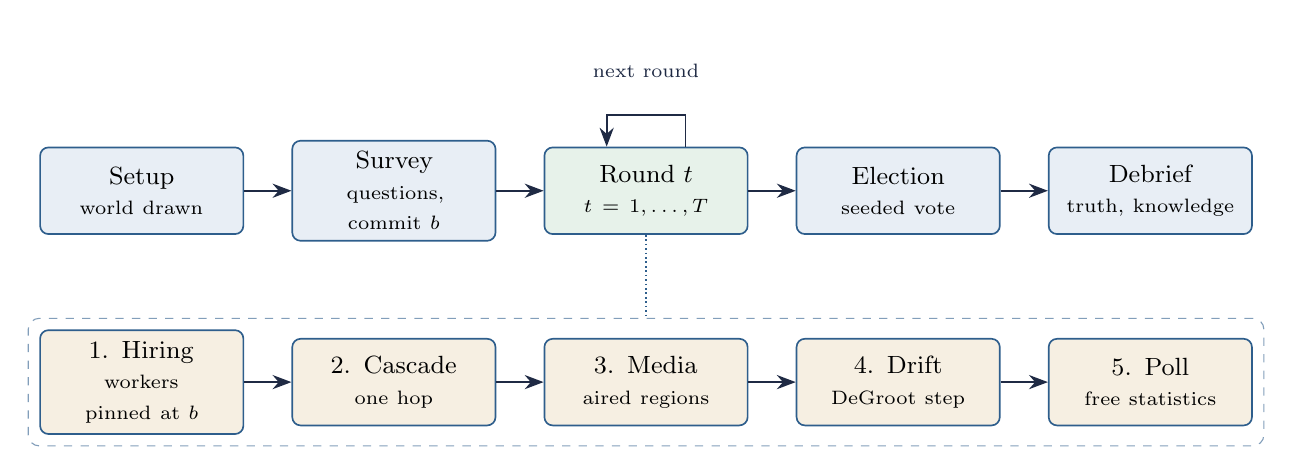
\begin{tikzpicture}[node distance=5mm and 6mm,
    every node/.append style={minimum height=11mm}]
  \node[box,text width=2.3cm] (setup) {Setup\\{\scriptsize world drawn}};
  \node[box,text width=2.3cm,right=of setup] (survey) {Survey\\{\scriptsize questions, commit $b$}};
  \node[boxg,text width=2.3cm,right=of survey] (round) {Round $t$\\{\scriptsize $t = 1,\dots,T$}};
  \node[box,text width=2.3cm,right=of round] (elec) {Election\\{\scriptsize seeded vote}};
  \node[box,text width=2.3cm,right=of elec] (debrief) {Debrief\\{\scriptsize truth, knowledge}};
  \draw[arr] (setup) -- (survey);
  \draw[arr] (survey) -- (round);
  \draw[arr] (round) -- (elec);
  \draw[arr] (elec) -- (debrief);
  \draw[arr] ([xshift=5mm]round.north) -- ++(0,4mm) -| node[pos=0.25,above,font=\scriptsize]{next round}
             ([xshift=-5mm]round.north);
  \node[boxs,text width=2.3cm,below=12mm of setup] (r1) {1. Hiring\\{\scriptsize workers pinned at $b$}};
  \node[boxs,text width=2.3cm,right=of r1] (r2) {2. Cascade\\{\scriptsize one hop}};
  \node[boxs,text width=2.3cm,right=of r2] (r3) {3. Media\\{\scriptsize aired regions}};
  \node[boxs,text width=2.3cm,right=of r3] (r4) {4. Drift\\{\scriptsize DeGroot step}};
  \node[boxs,text width=2.3cm,right=of r4] (r5) {5. Poll\\{\scriptsize free statistics}};
  \draw[arr] (r1) -- (r2);
  \draw[arr] (r2) -- (r3);
  \draw[arr] (r3) -- (r4);
  \draw[arr] (r4) -- (r5);
  \begin{scope}[on background layer]
    \node[draw=accent!60,dashed,rounded corners=4pt,fit=(r1)(r5),inner sep=4pt,minimum height=0pt] (inner) {};
  \end{scope}
  \draw[densely dotted,line width=0.6pt,color=accent] (round.south) -- (inner.north -| round.south);
\end{tikzpicture}
\caption{The phases of a game (top) and the order of events inside one campaign round (bottom).}
\label{fig:flow}
\end{figure}

\section{Actions}

The player has four kinds of action (\cref{tab:actions}). Every action is checked by the game before it
takes effect. An action that breaks a rule, such as spending more than the treasury holds or committing a
budget that does not sum to one, is rejected with an error code. A rejected action changes nothing and
costs nothing.

\begin{table}[t]
\centering
\caption{The player's actions. Media prices scale with region size; \coins{50} is the price for a region
holding a quarter of the voters.}
\label{tab:actions}
\small
\begin{tabularx}{\linewidth}{@{}l l l X@{}}
\toprule
Action & Phase & Cost & Effect \\
\midrule
\code{query}$(s_1,s_2,r)$ & survey, rounds & \coins{10} &
  Share of a fresh 10\% sample of region $r$ preferring sector $s_2$ over $s_1$, with a margin of error. \\
\code{commit}$(b)$ & survey & free &
  Fixes the manifesto $b$ for the rest of the game and starts round 1. \\
\code{allocate}$(h, m)$ & rounds & \coins{20} per worker, plus media &
  Hires $h_r$ new permanent workers in each region $r$ and airs media in the regions where $m_r$ is true;
  then the round is resolved. \\
\code{forfeit} & rounds & free & An allocation that buys nothing. \\
\bottomrule
\end{tabularx}
\end{table}

\paragraph{Party workers.} A worker is a real voter of the chosen region who joins the party. Their
preference is set to the manifesto and never changes again. Each new worker tries once to convert each of
their friends, and every voter they convert tries to convert their own friends in the next round. Workers
are therefore an investment: a worker hired early reaches further than one hired late.

\paragraph{Media.} A media airing reaches a share of the voters in one region and pulls each of them a
little towards the manifesto. Repeated airings in the same region have diminishing returns.

\paragraph{Survey questions.} Surveys are the only way to learn about the hidden regions. Each answer is an
estimate from a random sample, so it is noisy, and the same question may be asked again for a fresh
sample.

\section{Sequence of a game}

\Cref{fig:sequence} shows the messages exchanged during one game between the player (a person in a
browser, or a computer player), the game engine behind its API, and the simulation core that holds the
hidden electorate. The player only ever receives an \emph{observation}: an allow-listed summary that
contains no hidden information.

\begin{figure}[t]
\centering
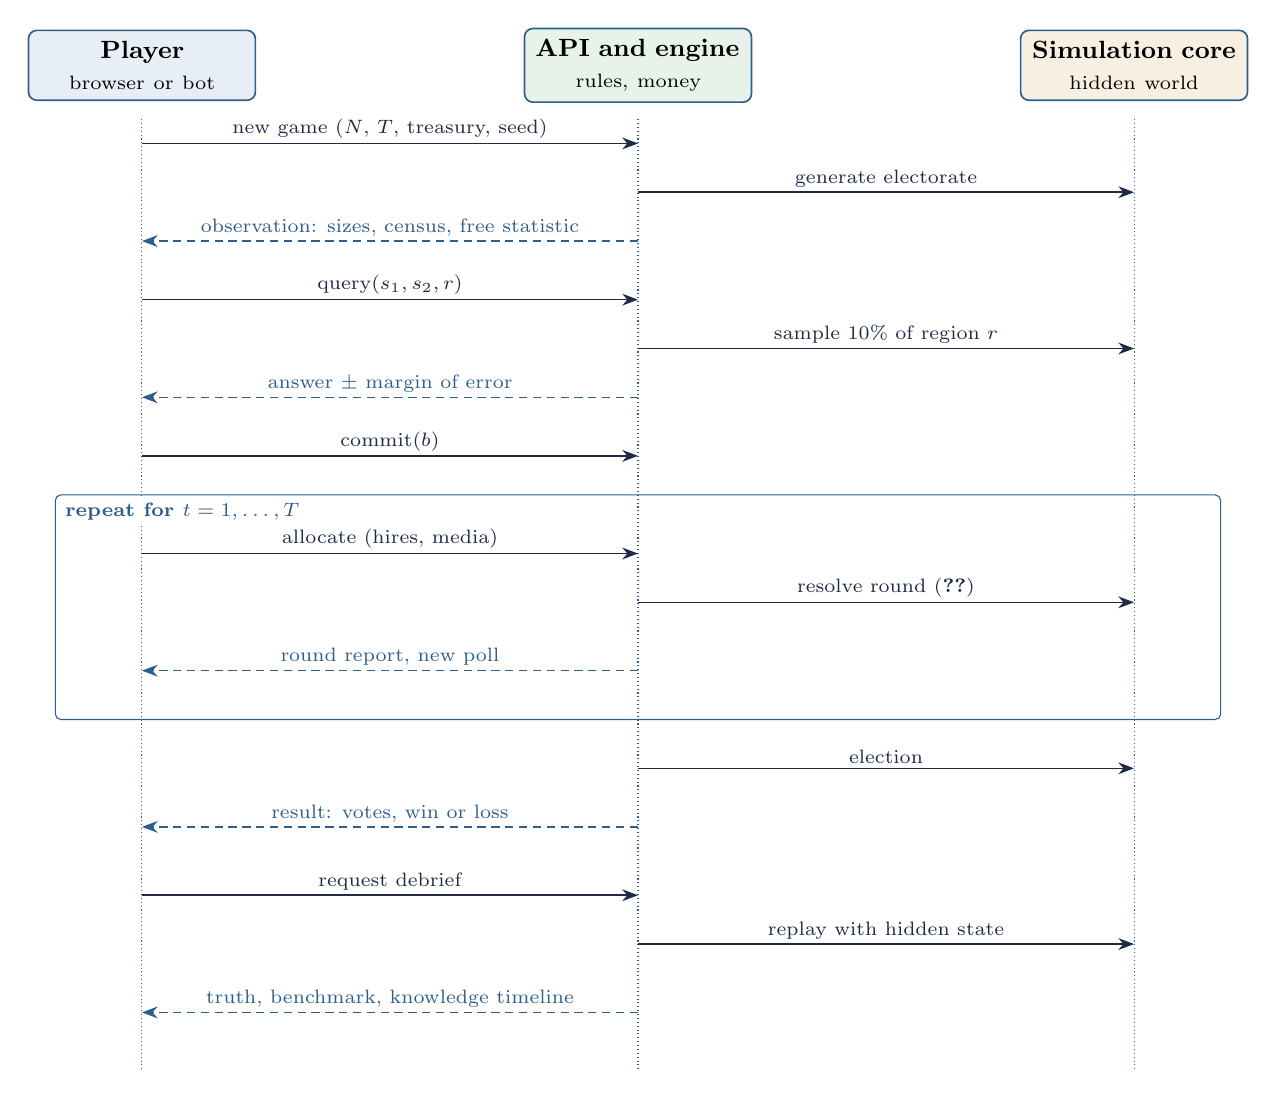
\begin{tikzpicture}[yscale=0.62]
  \def\xa{0} \def\xb{6.3} \def\xc{12.6}
  \node[box,text width=2.6cm] (P) at (\xa,0) {\textbf{Player}\\{\scriptsize browser or bot}};
  \node[boxg,text width=2.6cm] (G) at (\xb,0) {\textbf{API and engine}\\{\scriptsize rules, money}};
  \node[boxs,text width=2.6cm] (C) at (\xc,0) {\textbf{Simulation core}\\{\scriptsize hidden world}};
  \foreach \x in {\xa,\xb,\xc} \draw[densely dotted,color=accent] (\x,-1.1) -- (\x,-20.6);
  \tikzset{lab/.style={font=\scriptsize,above,inner sep=1.5pt}}
  \draw[msg] (\xa,-1.6) -- node[lab]{new game ($N$, $T$, treasury, seed)} (\xb,-1.6);
  \draw[msg] (\xb,-2.6) -- node[lab]{generate electorate} (\xc,-2.6);
  \draw[ret] (\xb,-3.6) -- node[lab]{observation: sizes, census, free statistic} (\xa,-3.6);
  \draw[msg] (\xa,-4.8) -- node[lab]{query$(s_1,s_2,r)$} (\xb,-4.8);
  \draw[msg] (\xb,-5.8) -- node[lab]{sample 10\% of region $r$} (\xc,-5.8);
  \draw[ret] (\xb,-6.8) -- node[lab]{answer $\pm$ margin of error} (\xa,-6.8);
  \draw[msg] (\xa,-8.0) -- node[lab]{commit$(b)$} (\xb,-8.0);
  % loop
  \draw[accent,rounded corners=2pt] (-1.1,-8.8) rectangle (13.7,-13.4);
  \node[font=\scriptsize\bfseries,color=accent,anchor=north west,fill=white,inner sep=2pt]
       at (-1.05,-8.85) {repeat for $t=1,\dots,T$};
  \draw[msg] (\xa,-10.0) -- node[lab]{allocate (hires, media)} (\xb,-10.0);
  \draw[msg] (\xb,-11.0) -- node[lab]{resolve round (\cref{alg:round})} (\xc,-11.0);
  \draw[ret] (\xb,-12.4) -- node[lab]{round report, new poll} (\xa,-12.4);
  \draw[msg] (\xb,-14.4) -- node[lab]{election} (\xc,-14.4);
  \draw[ret] (\xb,-15.6) -- node[lab]{result: votes, win or loss} (\xa,-15.6);
  \draw[msg] (\xa,-17.0) -- node[lab]{request debrief} (\xb,-17.0);
  \draw[msg] (\xb,-18.0) -- node[lab]{replay with hidden state} (\xc,-18.0);
  \draw[ret] (\xb,-19.4) -- node[lab]{truth, benchmark, knowledge timeline} (\xa,-19.4);
\end{tikzpicture}
\caption{Sequence of one game. Solid arrows are requests, dashed arrows are replies. The player never
talks to the simulation core directly.}
\label{fig:sequence}
\end{figure}

\section{Objects we had to build}

The game needs a small number of carefully separated objects (\cref{fig:objects}). The separation matters
because the whole point of the game is that the player does not see the hidden state.
\begin{itemize}
  \item \textbf{Game configuration}: every rule, price and parameter, plus $N$, $T$, the treasury and the
        seed. It is immutable once the game is created.
  \item \textbf{Electorate}: the hidden world. It holds the friendship graph, the region of each voter,
        each voter's preference and susceptibilities, the zealots, and the hidden archetype and
        personality maps. It is described in \cref{ch:electorate}.
  \item \textbf{Game state}: an immutable snapshot of the whole game: phase, round, the current
        preferences of all voters, one player state per player, the counters of the random streams and an
        event log. Every accepted action produces a new snapshot.
  \item \textbf{Player state}: the treasury (kept as exact decimals), the manifesto, the workers hired in
        each region, the number of media airings per region, and the knowledge log.
  \item \textbf{Knowledge log}: an append-only list of everything the player has observed (statistics,
        survey answers, polls and their own actions), each tagged with its round. It is the basis of the
        logic layer.
  \item \textbf{Observation}: the player's view, built from the game state by copying only allow-listed
        public fields. It is the only thing a player, human or computer, ever receives.
  \item \textbf{Action and allocation}: what the player sends back. An allocation lists the workers to hire
        per region and the regions to air media in.
\end{itemize}

\begin{figure}[t]
\centering
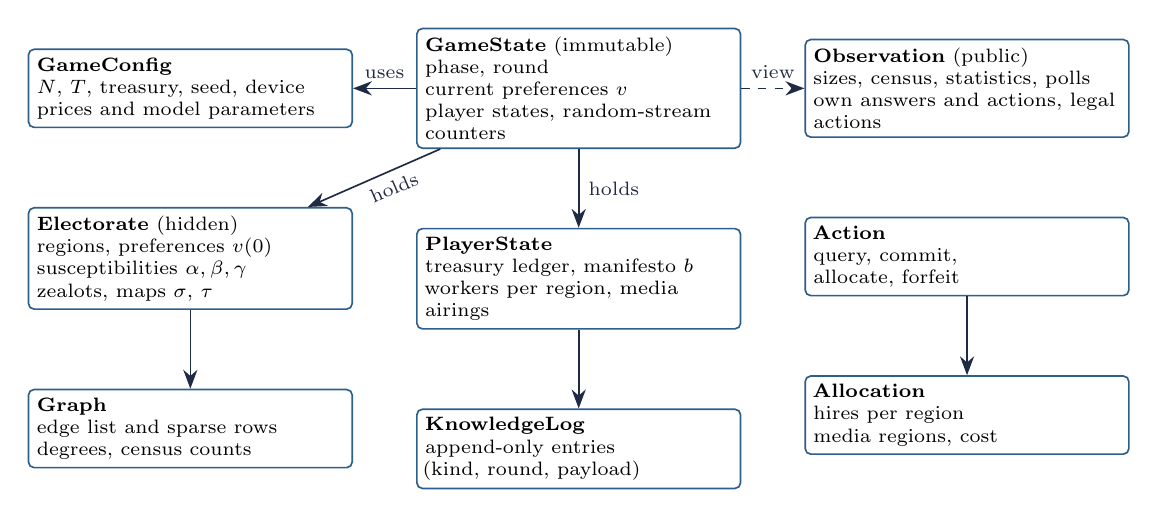
\begin{tikzpicture}[node distance=10mm and 8mm]
  \node[obj] (cfg) {\textbf{GameConfig}\\ $N$, $T$, treasury, seed, device\\ prices and model parameters};
  \node[obj,right=of cfg] (state) {\textbf{GameState} (immutable)\\ phase, round\\ current preferences $v$\\
        player states, random-stream counters};
  \node[obj,right=of state] (obs) {\textbf{Observation} (public)\\ sizes, census, statistics, polls\\
        own answers and actions, legal actions};
  \node[obj,below=of cfg] (elec) {\textbf{Electorate} (hidden)\\ regions, preferences $v(0)$\\
        susceptibilities $\alpha,\beta,\gamma$\\ zealots, maps $\sigma$, $\tau$};
  \node[obj,below=of state] (pst) {\textbf{PlayerState}\\ treasury ledger, manifesto $b$\\
        workers per region, media airings};
  \node[obj,below=of obs] (act) {\textbf{Action}\\ query, commit,\\ allocate, forfeit};
  \node[obj,below=of elec] (graph) {\textbf{Graph}\\ edge list and sparse rows\\ degrees, census counts};
  \node[obj,below=of pst] (klog) {\textbf{KnowledgeLog}\\ append-only entries\\ (kind, round, payload)};
  \node[obj,below=of act] (alloc) {\textbf{Allocation}\\ hires per region\\ media regions, cost};
  \draw[arr] (state) -- node[above,font=\scriptsize]{uses} (cfg);
  \draw[arr] (state) -- node[below,sloped,pos=0.4,font=\scriptsize]{holds} (elec);
  \draw[arr] (state) -- node[right,font=\scriptsize]{holds} (pst);
  \draw[arr,dashed] (state) -- node[above,font=\scriptsize]{view} (obs);
  \draw[arr] (elec) -- (graph);
  \draw[arr] (pst) -- (klog);
  \draw[arr] (act) -- (alloc);
\end{tikzpicture}
\caption{The main objects of the game. Arrows point from an object to what it holds or uses; the dashed
arrow is the allow-listed view that turns the hidden state into a player's observation.}
\label{fig:objects}
\end{figure}

\section{The voting mechanism}

In the spatial theory of voting, each voter has an ideal point in a space of
policies and prefers the platform closest to it. Our voters' ideal points are budget splits, so the space
of policies is the probability simplex
\begin{equation}
  \simplex = \Bigl\{\, x \in \R^5 : x_k \ge 0,\ \textstyle\sum_{k} x_k = 1 \,\Bigr\}.
\end{equation}
We measure how far apart two budget splits are by the \emph{total-variation} distance
$\TV(x,y)=\tfrac12\lVert x-y\rVert_1$: the share of the budget that would have to move to turn one split
into the other. Voter $i$'s agreement with the manifesto $b$ is
\begin{equation}
  S_i = 1 - \tfrac12\,\lVert v_i - b \rVert_1 \in [0,1].
\end{equation}
Instead of a hard ``closest platform wins'' rule, a voter supports the party with a probability that rises
smoothly with agreement (\cref{fig:vote}):
\begin{equation}\label{eq:vote}
  P_i = \sig\bigl(\beta_v\,(S_i - z)\bigr) = \frac{1}{1+\exp\bigl(-\beta_v\,(S_i - z)\bigr)},
  \qquad \beta_v = 20,\quad z = 0.825 .
\end{equation}
A voter whose agreement equals the threshold $z$ votes for the party half the time, and the slope $\beta_v$
sets how sharply support rises around it. We call
\begin{equation}
  E = \frac{1}{N}\sum_{i=1}^{N} P_i
\end{equation}
the \emph{expected vote share}. It is what the player tries to raise, and the main quantity we analyse.
The official result is a seeded random draw in which each voter votes independently with probability
$P_i$. The party wins with more than $N/2$ votes; a tie is a loss.

\begin{figure}[t]
\centering
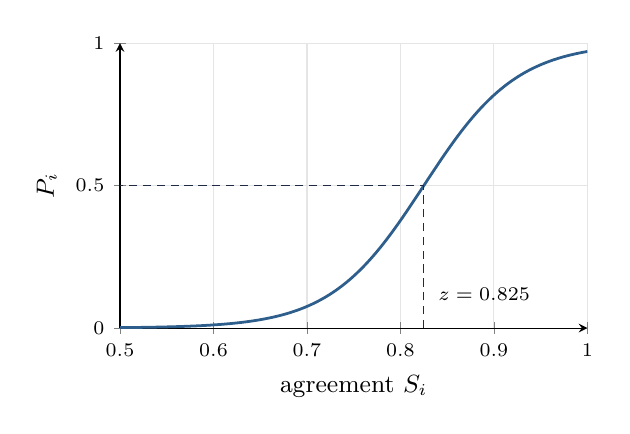
\begin{tikzpicture}
\begin{axis}[width=0.62\linewidth,height=5.2cm,
    xmin=0.5,xmax=1,ymin=0,ymax=1,
    xlabel={agreement $S_i$},ylabel={$P_i$},
    xtick={0.5,0.6,0.7,0.8,0.9,1},
    ytick={0,0.5,1},
    tick label style={font=\scriptsize},label style={font=\small},
    axis lines=left,grid=major,grid style={gray!20}]
  \addplot[domain=0.5:1,samples=120,line width=1pt,color=accent] {1/(1+exp(-20*(x-0.825)))};
  \draw[densely dashed,color=ink] (axis cs:0.825,0) -- (axis cs:0.825,0.5) -- (axis cs:0.5,0.5);
  \node[font=\scriptsize,anchor=west] at (axis cs:0.83,0.12) {$z = 0.825$};
\end{axis}
\end{tikzpicture}
\caption{Probability of voting for the party as a function of agreement with the manifesto
($\beta_v = 20$, $z = 0.825$). A voter must agree on more than 82.5\% of the budget to lean towards the
party.}
\label{fig:vote}
\end{figure}

\section{What the player can see}

The information model separates three kinds of facts.
\begin{description}[leftmargin=0pt,style=nextline]
  \item[Public at all times.] The rules and prices, $N$ and $T$, the size of each region, the archetype
        and personality libraries of \cref{ch:electorate} (but not which region has which), the player's
        own treasury and actions, and a network census: the number of friendships inside each region and
        between each pair of regions.
  \item[Free each round.] For every sector, the share of all voters who rank it in their top three, and a
        national poll of 400 random voters with its 95\% margin of error.
  \item[Paid, \coins{10} each.] A survey question ``in region $r$, what share of voters prefer sector $s_2$
        over sector $s_1$?'', answered from a fresh random sample of 10\% of the region with its margin of
        error. Repeated answers within a round are also pooled.
\end{description}
Everything else stays hidden: which archetype and personality each region has, the graph, every
individual preference and susceptibility, the zealots and all seeds. A world is \emph{consistent} with
the player's knowledge log if replaying the player's own actions in that world would have produced the
same observations. The set of consistent worlds is the player's \emph{information set}, the starting
point of \cref{ch:logic}.

\section{The system update}

\Cref{alg:round} is the heart of the game: what happens when a round's allocation is submitted. Its five
steps follow the order of \cref{fig:flow}. Every random draw comes from a named stream keyed by the round
and the player, so the same seed and the same actions always reproduce the same game.

\begin{algorithm}[t]
\caption{Resolve campaign round $t$ for a player with manifesto $b$}\label{alg:round}
\begin{algorithmic}[1]
\Require state $(v, \text{workers}, \text{converts}_{t-1}, \text{attempts}, \text{airings})$, allocation
         $(h, m)$
\State check that the allocation is valid and affordable; deduct its cost from the treasury
\For{each region $r$} \Comment{1. hiring}
  \State pick $h_r$ random eligible voters of $r$ (degree $\ge 3$, not a zealot, not a worker)
  \State mark them as workers and set their preference to $b$
\EndFor
\State spreaders $\gets$ new workers $\cup$ converts$_{t-1}$ \Comment{2. one cascade hop}
\State $P_j \gets \sig(\beta_v(S_j - z))$ for every voter, from the current preferences
\State converts$_t$ $\gets$ \Call{CascadeHop}{spreaders, $P$, attempts} \Comment{\cref{alg:cascade}}
\State set $v_j \gets b$ for every $j \in$ converts$_t$
\State $c_i \gets$ media pull on each voter of the aired regions; airings$_r$ += 1 \Comment{3. media}
\State $v \gets$ \Call{SocialStep}{$v$, $c$, $b$}; keep workers at $b$ and zealots fixed
       \Comment{4. drift, \cref{eq:update}}
\State draw a 400-voter poll and the top-three statistic; log both
       \Comment{5. poll}
\If{$t = T$} run the election \EndIf
\end{algorithmic}
\end{algorithm}

\section{Design choices and calibration}

Several rules above were chosen deliberately, and the default values were tuned before any experiment.
\begin{itemize}
  \item \textbf{Calibration.} Some parameter choices make the game either trivial or hopeless. A
        calibration study on 200 seeds tuned the voter concentration, the social step, the media strength,
        and the voting slope and threshold until a uniform manifesto with no campaign rarely won and a
        well-informed campaign usually did.
  \item \textbf{Workers are an investment.} There are no free workers: each worker is bought once, is a real
        voter of the network, stays pinned at the manifesto, and spreads influence one hop per round. A
        worker hired early therefore reaches further than one hired late, and the value of a worker depends
        on the network around it.
  \item \textbf{Prices and choices.} A worker costs \coins{20} and a survey question \coins{10}; the
        treasury is the player's choice; and the web game limits $T$ to 3--5 rounds so that games are neither
        too short to campaign nor so long that drift alone decides them.
  \item \textbf{Noisy surveys.} Survey answers are estimates from a 10\% sample rather than exact regional
        shares, so information is uncertain and repeating a question can be worthwhile.
\end{itemize}

\summarysection

A game moves through setup, a survey phase that ends with committing a manifesto, $T$ campaign rounds and
an election. The player can ask survey questions, commit, allocate money to workers and media, or skip a
round, and every action is validated before it takes effect. The game is built from a few separated
objects: an immutable configuration, a hidden electorate, immutable game states, player states with a
knowledge log, and allow-listed observations. Voters vote with a probability that rises steeply once their
agreement with the manifesto passes 0.825, and each round is resolved by the five steps of
\cref{alg:round}. The next chapter describes the electorate.

%% =====================================================================
%%  Chapter 3: Electorate
%% =====================================================================
\chapter{The Electorate}\label{ch:electorate}

\overviewsection

The electorate is the hidden world the player is trying to win over. This chapter describes how it is
generated: the regions, the friendship network, what voters want, how easily they can be moved, and the
zealots who cannot be moved at all. It then describes how opinions change from round to round, and the
theory that predicts how fast. The background on each model is given where it is used.

\section{Regions}

The $N$ voters are split into four regions, North, South, East and West. Every region holds at least 15\%
of the voters, and the rest are split at random. With $m=\lceil 0.15N\rceil$,
\begin{equation}
  \pi \sim \operatorname{Dirichlet}(2,2,2,2), \qquad
  n_r = m + \bigl[\operatorname{Multinomial}(N-4m,\ \pi)\bigr]_r ,
\end{equation}
so $\sum_r n_r = N$ and $n_r \ge m$ for every region. Region sizes are public.

\section{The friendship network}

A social network is a graph whose nodes are people and whose edges are friendships. We write $A$ for its
adjacency matrix, $d_i$ for the degree of voter $i$ and $D$ for the diagonal matrix of degrees. The
simplest random graph links every pair independently with the same probability, but real
societies have more friends inside their own community. The \emph{stochastic block model}
captures this by splitting nodes into blocks and letting the link probability depend on the pair of blocks.
Our blocks are the four regions (\cref{fig:sbm}).

For each game we draw ten connection weights: one inside each region, $p_r \sim U[0.5, 0.9]$, and one for
each pair of regions, $p_{rs} \sim U[0.01, 0.2]$. Used directly they would make the graph almost complete,
so all of them are scaled by one sparsity factor $s$ that keeps their ratios but sets the expected mean
degree to $\bar k = 30$:
\begin{equation}
  P_{rr} = s\,p_r, \qquad P_{rs} = s\,p_{rs}, \qquad
  s = \frac{\bar k\,N}{\sum_r p_r\,n_r(n_r-1) + \sum_{r\neq s} p_{rs}\,n_r n_s}.
\end{equation}
Inside each block every pair of voters is linked independently with probability $P$. With typical draws
about three quarters of a voter's friends live in their own region. Edges are unweighted. The player sees
the number of friendships inside and between regions, but never the edges.

\begin{figure}[t]
\centering
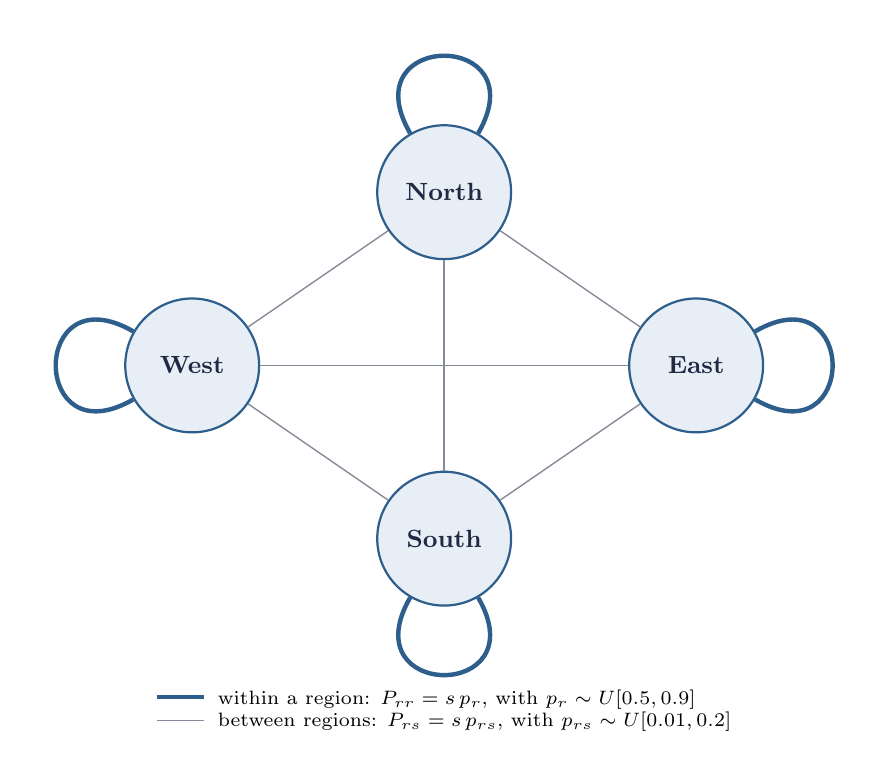
\begin{tikzpicture}[region/.style={circle,draw=accent,line width=0.8pt,fill=soft,minimum size=17mm,
                                   font=\small\bfseries,text=ink},
                    weak/.style={line width=0.5pt,color=ink!55},
                    strong/.style={line width=1.6pt,color=accent}]
  \node[region] (N) at (0,2.2) {North};
  \node[region] (S) at (0,-2.2) {South};
  \node[region] (E) at (3.2,0) {East};
  \node[region] (W) at (-3.2,0) {West};
  \foreach \a/\b in {N/S,N/E,N/W,S/E,S/W,E/W} \draw[weak] (\a) -- (\b);
  \draw[strong] (N) to[out=60,in=120,looseness=4.5] (N);
  \draw[strong] (S) to[out=-60,in=-120,looseness=4.5] (S);
  \draw[strong] (E) to[out=30,in=-30,looseness=4.5] (E);
  \draw[strong] (W) to[out=150,in=210,looseness=4.5] (W);
  \node[font=\scriptsize,anchor=north,align=left] at (0,-4.0)
       {\textcolor{accent}{\rule[2pt]{6mm}{1.6pt}}\; within a region: $P_{rr} = s\,p_r$, with $p_r \sim U[0.5,0.9]$\\
        \textcolor{ink!55}{\rule[2pt]{6mm}{0.5pt}}\; between regions: $P_{rs} = s\,p_{rs}$, with $p_{rs} \sim U[0.01,0.2]$};
\end{tikzpicture}
\caption{The friendship network is a stochastic block model whose blocks are the regions. Links are much
more likely inside a region than between regions.}
\label{fig:sbm}
\end{figure}

\section{What voters want: archetypes}

Each voter $i$ holds a preferred budget split $v_i \in \simplex$ over the five sectors, in the order
education, welfare, agriculture, industry, environment. Regions differ in what they want. There is a
public library of six \emph{archetypes} (\cref{tab:archetypes}), and a hidden one-to-one map $\sigma$
gives one archetype to each region; there are $6\cdot5\cdot4\cdot3 = 360$ such maps. A voter in region $r$
starts at
\begin{equation}
  v_i(0) \sim \operatorname{Dirichlet}\bigl(\kappa\,\mu_{\sigma(r)}\bigr), \qquad \kappa = 60,
\end{equation}
so voters of one region want similar but not identical things; a larger $\kappa$ would make them more
alike.

\begin{table}[t]
\centering
\caption{The public archetype library. Each row is the mean budget split $\mu$ of one archetype.}
\label{tab:archetypes}
\small
\begin{tabular}{@{}llccccc@{}}
\toprule
ID & Name & Education & Welfare & Agriculture & Industry & Environment \\
\midrule
A0 & Agrarian heartland & 0.15 & 0.20 & 0.40 & 0.10 & 0.15 \\
A1 & Industrial belt    & 0.15 & 0.15 & 0.10 & 0.45 & 0.15 \\
A2 & Green urban        & 0.25 & 0.10 & 0.10 & 0.15 & 0.40 \\
A3 & Welfare-reliant    & 0.15 & 0.45 & 0.15 & 0.10 & 0.15 \\
A4 & Knowledge hub      & 0.40 & 0.10 & 0.10 & 0.25 & 0.15 \\
A5 & Balanced middle    & 0.20 & 0.20 & 0.20 & 0.20 & 0.20 \\
\bottomrule
\end{tabular}
\end{table}

\section{How voters can be moved: personalities}

Voters also differ in how easily they are moved. Each voter has three susceptibilities in $[0,1]$: to
friends ($\alpha_i$), to media ($\beta_i$) and to canvassing by party workers ($\gamma_i$). Each region has
one of four public \emph{personalities} (\cref{tab:personalities}), assigned by a hidden permutation $\tau$
(24 possibilities), and its voters draw their susceptibilities from that personality's Beta distributions.

\begin{table}[t]
\centering
\caption{The public personality library. Voters draw their susceptibilities from the Beta distributions
of their region's personality.}
\label{tab:personalities}
\small
\begin{tabular}{@{}llccc@{}}
\toprule
ID & Name & Friends $\alpha$ & Media $\beta$ & Canvassing $\gamma$ \\
\midrule
P0 & Socially driven         & Beta(6,3) & Beta(2,5) & Beta(3,4) \\
P1 & Media-savvy             & Beta(3,4) & Beta(6,3) & Beta(2,5) \\
P2 & Independent             & Beta(2,6) & Beta(2,6) & Beta(2,6) \\
P3 & Receptive to canvassing & Beta(3,4) & Beta(3,4) & Beta(6,3) \\
\bottomrule
\end{tabular}
\end{table}

\section{Zealots}

Each voter is independently a \emph{zealot} with probability $\zeta = 0.05$. Zealots never change their
mind ($\alpha=\beta=\gamma=0$), but their friends still listen to them. In opinion dynamics, such
\emph{stubborn agents} are known to have outsized effects: a single zealot can pull a whole population
towards their view, and zealots who disagree prevent consensus altogether.
Our zealots keep the electorate from collapsing to a single opinion, and they cannot be hired or
converted.

\section{The hidden type of a world}

The pair $\theta = (\sigma,\tau)$ is the \emph{hidden type} of a world; there are $360 \times 24 = 8640$
of them. Everything else, the graph, the individual preferences, the susceptibilities and the zealots, is
the \emph{micro-state}. Survey answers depend only on preferences, which depend only on $\sigma$, so
surveys can reveal $\sigma$ but not $\tau$; the player can learn about personalities only indirectly,
through polls. \Cref{alg:electorate} summarises how a world is generated.

\begin{algorithm}[t]
\caption{Generate an electorate from $(N, \text{seed})$}\label{alg:electorate}
\begin{algorithmic}[1]
\State derive named random streams (regions, graph, preferences, attributes, zealots) from the seed
\State draw region sizes $n_r$ with the 15\% floor
\State draw $p_r$, $p_{rs}$; compute $s$; for each block, draw the number of edges, then their endpoints;
       remove self-loops and duplicates
\State draw a random archetype map $\sigma$ and personality map $\tau$
\For{each voter $i$ in region $r$}
  \State $v_i(0) \sim \operatorname{Dirichlet}(\kappa\,\mu_{\sigma(r)})$
  \State $\alpha_i,\beta_i,\gamma_i \sim$ Beta distributions of personality $\tau(r)$
  \State with probability $\zeta$: make $i$ a zealot ($\alpha_i=\beta_i=\gamma_i=0$)
\EndFor
\State \Return graph, regions, $v(0)$, susceptibilities, zealots, $\sigma$, $\tau$
\end{algorithmic}
\end{algorithm}

All of this is done with tensor operations, block by block, so memory grows with the number of edges and
a million-voter electorate takes a few seconds to build. The electorate is drawn on the CPU and then moved
to the GPU, so the same $N$ and seed give exactly the same world on any machine.

\section{How opinions change}

\subsection{DeGroot averaging}

In the DeGroot model, each person repeatedly replaces their opinion with the average of
their neighbours' opinions, $x(t+1) = W x(t)$ with $W = D^{-1}A$. On a connected graph that is not
bipartite, opinions converge to a common value. The speed is governed by the second-largest eigenvalue
modulus $\mu_2$ of $W$: disagreement shrinks roughly like $\mu_2^{\,t}$. A
closely related measure is the algebraic connectivity, the second-smallest eigenvalue of the Laplacian
$L = D - A$. A graph with weak links between communities, like ours, has $\mu_2$ close
to 1 and converges slowly.

\subsection{The update rule}

Our voters do not average completely each round. Let $a_i = \omega\,\alpha_i$ with $\omega = 0.15$ be the
weight voter $i$ gives to friends, and $c_i$ the combined campaign pull on $i$ this round. All voters
update at the same time:
\begin{equation}\label{eq:update}
  v_i \leftarrow (1 - a_i - c_i)\,v_i \;+\; a_i\,\bar v_{\mathcal N(i)} \;+\; c_i\, b,
  \qquad
  \bar v_{\mathcal N(i)} = \frac{1}{d_i}\sum_{j \in \mathcal N(i)} v_j ,
\end{equation}
where $\mathcal N(i)$ is the set of $i$'s friends. If $a_i + c_i$ would exceed 1, the campaign pull is
scaled down so that it does not. The new preference is a convex combination of points of the simplex, so
it stays in the simplex. Zealots do not update, and party workers are reset to $b$ after every step.

\subsection{Stubborn agents and resilient averaging}

Party workers never change their view, so from the network's point of view they are stubborn agents placed
by the party. In the Friedkin--Johnsen model, agents who keep some attachment to a
fixed opinion make the population settle at an equilibrium instead of a consensus, and stubborn agents
pull that equilibrium towards their own view. Over a long horizon, pinned workers would therefore drag
their region towards the manifesto even without any cascade.

\emph{Resilient consensus} asks how normal agents can still agree when some agents misbehave. In the W-MSR
algorithm, each agent discards the $F$ most extreme neighbour values before averaging;
it works when the graph is sufficiently \emph{robust}, a property that is hard to check exactly. We
implemented W-MSR on the simplex (neighbours are ranked by their TV distance) as an alternative to plain
averaging. It acts as a possible defence of the network against the campaign's stubborn workers, and we
also compute bounds on the graph's robustness. Bounded-confidence models are another
well-known variant, which we did not implement.

\summarysection

An electorate is four regions of voters linked by a stochastic block model with mean degree 30 and strong
ties inside regions. Each region has a hidden archetype (what it wants) and a hidden personality (how it
can be moved), and 5\% of voters are zealots. Together the two hidden maps give 8640 world types. Each
round voters move part of the way towards the average of their friends, a damped DeGroot step whose speed
is set by the spectrum of the network, while workers act as stubborn agents. The next chapter gives the
algorithms that act on this electorate.

%% =====================================================================
%%  Chapter 4: Algorithms
%% =====================================================================
\chapter{Algorithms}\label{ch:algorithms}

\overviewsection

This chapter gives the algorithms of the game, in two groups. The first group is the campaign mechanics:
the worker cascade and media. The second group is decision making: how a player keeps a belief about the
hidden world, chooses which question to ask, picks a manifesto, and plans its spending. We end with the
reference algorithms we use to judge how well a player does, and with the computer players built from all
of these.

\section{The worker cascade}

\subsection{Background}

In the \emph{Independent Cascade} model, when a node becomes active it gets
one chance to activate each inactive neighbour $j$, and succeeds with some probability $q_j$. Newly
activated nodes get their own chance in the next step. Whether the cascade dies out or spreads depends on
an \emph{epidemic threshold}: the spectral radius of the adjacency matrix weighted by the transmission
probabilities. If each neighbour $j$ converts with probability $q_j$, the
expected number of new activations grows by the operator $A\,D_q$ with $D_q=\operatorname{diag}(q)$, and
the cascade grows when $\lambda_{\max}(A D_q) > 1$.

Influence maximisation asks which $k$ seeds give the largest expected spread. Under the Independent
Cascade the spread is a \emph{submodular} function of the seed set: each new seed adds less than the
previous one. For such functions the greedy algorithm reaches at least $1-1/e$ of the
optimum, and the CELF algorithm makes greedy selection much faster by updating
marginal gains lazily. Our workers are the seeds of such a cascade.

\subsection{Our cascade}

The spreaders of round $t$ are the workers hired in round $t$ and the voters converted in round $t-1$. Each
spreader tries once to convert each friend $j$ (workers and zealots cannot be targeted). If $j$ receives
$e_j$ attempts this round, it converts with probability
\begin{equation}\label{eq:convert}
  1 - \bigl(1 - \gamma_j P_j\bigr)^{e_j},
\end{equation}
where $P_j$ is $j$'s current probability of voting for the party (\cref{eq:vote}). No voter may receive more
than three attempts in the whole game, failures included. A convert jumps to $v_j = b$, spreads in the next
round only, and is an ordinary voter afterwards. \Cref{alg:cascade} gives one hop; it is computed for all
voters at once with sparse edge counts, never with a loop over voters.

\begin{algorithm}[t]
\caption{\textsc{CascadeHop}: one round of the worker cascade}\label{alg:cascade}
\begin{algorithmic}[1]
\Require spreaders $\mathcal S$, vote probabilities $P$, attempts used so far $u$, cap $3$
\For{every voter $j$ that is not a worker or a zealot} \Comment{done in parallel}
  \State $k_j \gets$ number of edges from $\mathcal S$ to $j$
  \State $e_j \gets \min(k_j,\ 3 - u_j)$; \quad $u_j \gets u_j + e_j$
  \State $q_j \gets 1 - (1 - \gamma_j P_j)^{e_j}$
  \State $j$ converts with probability $q_j$
\EndFor
\State \Return the set of converts
\end{algorithmic}
\end{algorithm}

The factor $P_j$ in \cref{eq:convert} is a deliberate choice: voters who already lean towards the manifesto
are easier to convert. It also couples the two halves of the game. A manifesto close to what a region wants
raises $P_j$ there, which raises $q_j = \gamma_j P_j$ and can push that region above its epidemic
threshold $\lambda_{\max}(A D_q) = 1$. The manifesto is not only a policy choice; it also decides how far
the party's workers can reach.

\section{Media}

An airing in region $r$ costs $m_0\, n_r / (N/4)$ with $m_0 = 50$. Each voter of an aired region is reached
with probability $p_m = 0.6$, and a reached voter feels a pull towards $b$ of strength
\begin{equation}
  c_i = \eta_m(n)\,\beta_i, \qquad \eta_m(n) = \frac{\eta_0}{1+\lambda n},\quad \eta_0 = 0.25,\ \lambda = 0.5,
\end{equation}
where $n$ counts the player's earlier airings in that region. The pull enters the update of
\cref{eq:update}. Repeated airings therefore have diminishing returns, and media helps most in media-savvy
regions, where $\beta_i$ is large.

\section{Belief over the hidden world}

A player who does not know the hidden state faces a partially observable decision
problem, which is intractable to solve exactly at our scale. Our players use two
standard approximations: a Bayesian belief over hidden worlds, and planning by rollouts.

Survey answers depend only on $\sigma$. The belief is therefore an exact posterior over the 360
archetype maps, starting from a uniform prior, while the belief over $\tau$ stays uniform. For each archetype, the
distribution of answers to each question is precomputed once by Monte Carlo. When an answer $\hat a$
arrives, every map is reweighted by a Gaussian likelihood
\begin{equation}
  \Pr(\sigma \mid \hat a) \;\propto\; \Pr(\sigma)\,
  \exp\!\Bigl(-\frac{(\hat a - a_\sigma)^2}{2 s^2_\sigma}\Bigr),
\end{equation}
where $a_\sigma$ is the answer expected under $\sigma$ and $s_\sigma$ combines the sampling error of a 10\%
sample with the spread of answers across voters. The free top-three statistic is used in the same way.

\section{Choosing a survey question}

Bayesian experimental design suggests asking the question whose answer is expected to reduce uncertainty
most. For each of the $10 \times 4 = 40$ possible questions (a pair of
sectors and a region) the player computes the mutual information between the answer $Y$ and the map,
\begin{equation}
  I(\sigma; Y) = H(\sigma) - \E_{Y}\bigl[ H(\sigma \mid Y) \bigr],
\end{equation}
and asks the question with the largest value. It stops when the posterior entropy falls below 0.05 nats,
when the best question gains too little per coin, or after ten questions or \coins{50} of surveys. In a
campaign round it may ask one more question if the gain is large. Repeats are allowed, since each answer is
a fresh sample.

\section{Choosing the manifesto}

\subsection{The optimisation problem}

The manifesto should maximise the expected vote share on election day:
\begin{equation}\label{eq:manifesto}
  \max_{b \in \simplex}\ f(b) = \frac{1}{N}\sum_{i} \sig\!\Bigl(\beta_v\bigl(1 - \tfrac12\lVert v_i - b\rVert_1
  - z\bigr)\Bigr).
\end{equation}
An important lesson from calibration is that the electorate on election day is not the electorate at the
start: even without a campaign, social averaging pulls each region towards its mean. Every good player
therefore optimises against the \emph{anticipated} electorate, obtained by simulating $T$ rounds of
social-only dynamics. A player without full information does this on eight synthetic worlds built from its
posterior: each takes a map $\sigma$ sampled from the belief and draws everything else from the public
prior, at a reduced size of 1600 voters that keeps region proportions and degree structure.

The objective is neither smooth, because of the absolute values, nor concave. We replace $|x|$ by the
pseudo-Huber function $\sqrt{x^2+\delta^2}-\delta$ with a small $\delta$, and use several starts: the
uniform split, the population mean and the five vertices of the simplex pulled towards its centre. The best
start is chosen on the exact objective.

\subsection{Projected gradient}

Projected gradient takes a gradient step and then projects back onto the simplex (\cref{alg:pg}). The
Euclidean projection onto the simplex can be computed exactly in $O(n\log n)$ time. It is
the \emph{proximal operator} of the simplex's indicator function, so projected gradient is a special case
of the proximal gradient method.

\begin{algorithm}[t]
\caption{Multi-start projected gradient for the manifesto}\label{alg:pg}
\begin{algorithmic}[1]
\Require anticipated voters $\{v_i\}$, starts $b^{(0)}_1,\dots,b^{(0)}_M$, step $\eta$, smoothing $\delta$
\For{all starts $m$ in parallel}
  \Repeat
    \State $b_m \gets P_{\simplex}\bigl(b_m + \eta\,\nabla \tilde f_\delta(b_m)\bigr)$
           \Comment{$P_\simplex$: sort, threshold, clip}
  \Until{the change is below $10^{-4}$ or the iteration limit is reached}
\EndFor
\State \Return $\argmax_m f(b_m)$ on the exact, unsmoothed objective
\end{algorithmic}
\end{algorithm}

\subsection{Consensus ADMM}

ADMM splits a problem into pieces that are solved separately and then forced to agree. We
use it to solve \cref{eq:manifesto} as if each region negotiated its own preferred manifesto, the textbook
model of distributed optimisation in a multi-agent system. Write $-f(b) = \sum_r f_r(b)$, with $f_r$ region
$r$'s share weighted by its size. Each region keeps its own copy $x_r$, and a shared variable $z$ pulls the
copies together:
\begin{align}
  x_r &\leftarrow \argmin_{x}\ f_r(x) + \tfrac{\rho}{2}\,\lVert x - z + u_r \rVert^2, \\
  z   &\leftarrow P_{\simplex}\Bigl(\tfrac14 \textstyle\sum_r (x_r + u_r)\Bigr), \\
  u_r &\leftarrow u_r + x_r - z .
\end{align}
The first step is each region's local problem, solved inexactly with a few gradient steps. The second is
the projection that enforces agreement, and the third accumulates each region's disagreement. Because $f_r$
is not convex, ADMM reaches a stationary point and needs a fairly large penalty ($\rho = 5$) and a smoother
surrogate ($\delta = 0.02$) to avoid oscillating. We stop when both the primal residual
$\lVert x - z\rVert$ and the dual residual fall below $10^{-6}$.

\subsection{Other optimisers}

Two more first-order methods are implemented for comparison. \emph{Mirror descent} replaces Euclidean
geometry with the entropy, which gives multiplicative updates that stay inside the simplex
automatically. \emph{Frank--Wolfe} moves towards the vertex of the simplex that best
aligns with the gradient and needs no projection at all.

\section{Planning each round}

Planning uses rollouts: for each candidate action, simulate the rest of the game in
several worlds drawn from the belief, follow a fixed default policy afterwards, and pick the action with the
best average result (\cref{alg:rollout}). The candidate list holds at most twenty allocations built from
public information: doing nothing, workers only, media only and mixtures, all valid and affordable. The
default continuation is ``even'' pacing: each later round spends an equal share of the remaining money,
half on media in the least-aired regions and half on workers split by region size. All candidates are
simulated together in one batched call with common random numbers, so the differences between candidates
are not drowned out by noise.

\begin{algorithm}[t]
\caption{Rollout planning for round $t$}\label{alg:rollout}
\begin{algorithmic}[1]
\Require observation, belief over $\sigma$, number of worlds $B = 8$
\State $\mathcal C \gets$ up to 20 valid, affordable candidate allocations
\State sample $B$ worlds from the belief; in each, replay the player's past manifesto and allocations
\For{every candidate $a \in \mathcal C$ and world $w$, in one batch}
  \State play $a$ in round $t$, then the even continuation in rounds $t+1,\dots,T$
  \State $V[a,w] \gets$ expected vote share $E$ on election day
\EndFor
\State \Return $\argmax_{a} \frac1B \sum_w V[a,w]$
\end{algorithmic}
\end{algorithm}

\section{Reference algorithms}

To judge a player we need a target. We use two.

\paragraph{The full-information \ORACLE.} The \ORACLE{} is told every voter's true preference and
susceptibilities. It optimises the manifesto against the true anticipated electorate, and each round it
buys greedily by estimated gain in expected vote share per coin. For media this is the expected change in
$P_i$ over the voters who would be reached. For a worker in region $r$, it estimates the reach of a
cascade with per-attempt chance $a_r = \E_r[\gamma P]$ and mean degree $\bar k_r$ over the $L$ remaining
hops,
\begin{equation}
  \text{reach}_r \approx \min\Bigl(\bar k_r a_r \sum_{h=0}^{L-1} (\bar k_r a_r)^h,\ \tfrac12 n_r\Bigr),
\end{equation}
multiplied by the expected gain per converted voter. It is a sensible heuristic, but nothing guarantees
that it is optimal. Its results are always labelled and never mixed with those of fair players.

\paragraph{Plan search.} Given a manifesto and the true world, an open-loop search looks for the best
whole plan: how many workers and which media in each region, in each round. It uses the cross-entropy
method, which repeatedly samples plans, keeps the best fraction and refits the
sampling distribution to them (\cref{alg:cem}), followed by hill climbing. The final plan is re-scored on
20 fresh random streams so that its score is not inflated by the noise it was selected on. The search is
itself a heuristic, so its score is a lower bound on the best achievable.

\begin{algorithm}[t]
\caption{Cross-entropy plan search}\label{alg:cem}
\begin{algorithmic}[1]
\Require true world, manifesto $b$; 256 plans per iteration, elite fraction 10\%, smoothing 0.7
\State initialise a sampling distribution over per-round worker counts and media choices
\For{30 iterations}
  \State sample 256 affordable plans; simulate all of them in one batch
  \State keep the 26 best plans (the elite)
  \State refit the distribution to the elite, mixed 0.7 : 0.3 with the previous one
\EndFor
\State improve the best plan by hill climbing; re-score it on 20 fresh random streams
\end{algorithmic}
\end{algorithm}

\section{Computer players}

The players used in the experiments are built from these algorithms. All except the \ORACLE{} see only the
observation a human would see.
\begin{itemize}
  \item \textbf{Bayesian planner (player II)}: belief and question selection, manifesto by projected
        gradient (or by consensus ADMM in a variant), and rollout planning each round.
  \item \textbf{People Pleaser (player I)}: the same surveys and belief, then a rule of thumb. It picks the
        smallest group of largest regions that hold a majority, blends their most likely archetypes by
        size, and spends at an even pace with media in those regions and the rest on workers.
  \item \textbf{Strong-Arm (player III)}: asks nothing, pushes a fixed agenda, and spends half on media and
        half on workers at one and a half times the even pace, so its money runs out early.
  \item \textbf{Fixed patterns}: \emph{none}, \emph{all workers}, \emph{all media} and \emph{split} (half
        and half at an even pace), used to check balance.
  \item \textbf{Top-three and uniform}: one uses the free top-three statistic as its manifesto and spends
        evenly; the other commits the uniform split and never spends.
\end{itemize}
An interface for a language-model player also exists: it would receive the observation as JSON and reply
with one action. It is not implemented yet.

\summarysection

The worker cascade is an Independent Cascade with conversion chance $\gamma_j P_j$ and a cap of three
attempts per voter, so the manifesto itself moves regions across the epidemic threshold. Media gives a
diminishing pull in aired regions. Players keep an exact posterior over the 360 archetype maps, ask the
question with the largest expected information gain, optimise the manifesto on the simplex by projected
gradient or consensus ADMM against the anticipated electorate, and choose each round's spending by batched
rollouts. A full-information \ORACLE{} and a cross-entropy plan search serve as references. The next
chapter describes the software that runs all of this.

%% =====================================================================
%%  Chapter 5: System design and implementation
%% =====================================================================
\chapter{System Design and Implementation}\label{ch:system}

\overviewsection

This chapter describes the software. We start with the overall architecture, then explain the three
properties we cared about most: that every game can be replayed exactly, that the simulator runs fast
enough on a GPU to support large experiments, and that the player never sees hidden information. We then
describe the web game, the testing strategy and the experiment harness.

\section{Architecture}

\Cref{fig:arch} shows the layers. At the bottom, a \emph{simulation core} implements electorate
generation, dynamics, the campaign mechanics, voting and the information model as PyTorch
tensor operations. Above it, a \emph{game engine} enforces the rules: phases, validation, money and the
order of events in a round. Players and the reasoning layer talk to the engine, the experiment harness
drives the simulation core directly, and the web interface reaches the engine over an HTTP API.

\begin{figure}[t]
\centering
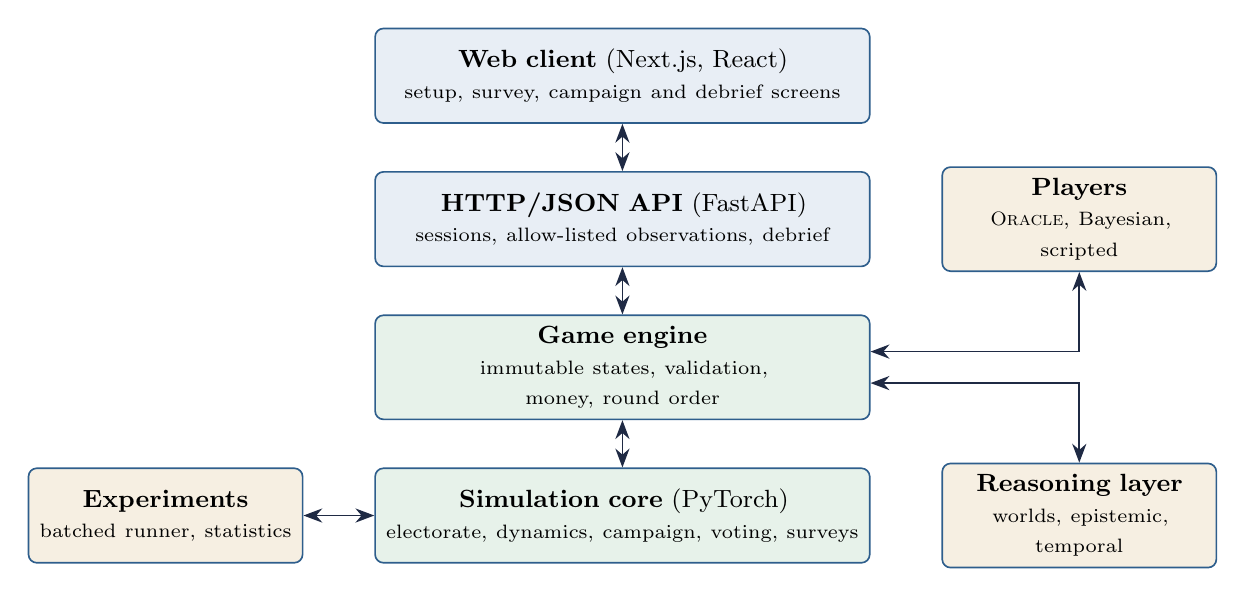
\begin{tikzpicture}[node distance=6mm and 9mm,
    every node/.append style={minimum height=12mm}]
  \node[box,text width=6.0cm] (web) {\textbf{Web client} (Next.js, React)\\
        {\scriptsize setup, survey, campaign and debrief screens}};
  \node[box,text width=6.0cm,below=of web] (api) {\textbf{HTTP/JSON API} (FastAPI)\\
        {\scriptsize sessions, allow-listed observations, debrief}};
  \node[boxg,text width=6.0cm,below=of api] (engine) {\textbf{Game engine}\\
        {\scriptsize immutable states, validation, money, round order}};
  \node[boxg,text width=6.0cm,below=of engine] (core) {\textbf{Simulation core} (PyTorch)\\
        {\scriptsize electorate, dynamics, campaign, voting, surveys}};
  \node[boxs,text width=3.2cm,right=of api] (players) {\textbf{Players}\\
        {\scriptsize \ORACLE, Bayesian, scripted}};
  \node[boxs,text width=3.2cm,right=of core] (logic) {\textbf{Reasoning layer}\\
        {\scriptsize worlds, epistemic, temporal}};
  \node[boxs,text width=3.2cm,left=of core] (exp) {\textbf{Experiments}\\
        {\scriptsize batched runner, statistics}};
  \draw[darr] (web) -- (api);
  \draw[darr] (api) -- (engine);
  \draw[darr] (engine) -- (core);
  \draw[darr] (players.south) |- ([yshift=2mm]engine.east);
  \draw[darr] (logic.north) |- ([yshift=-2mm]engine.east);
  \draw[darr] (exp) -- (core);
\end{tikzpicture}
\caption{Software architecture. Players and the reasoning layer see the game only through observations;
the experiment harness drives the simulation core directly for speed.}
\label{fig:arch}
\end{figure}

The code is a Python package with one module per concern: \code{electorate}, \code{dynamics},
\code{voting}, \code{information}, \code{game}, \code{strategies}, \code{logic}, \code{analysis} (spectral
and robustness tools) and \code{api}. The package has about 5,900 lines of Python, the web client about
5,600 lines of TypeScript, and the experiment scripts about 13,000 lines.

\section{The game engine}

The engine is a set of pure functions over immutable game states (\cref{fig:objects}). Applying an action
returns a new state; a rejected action returns the same state object with an error code (for example
\code{INSUFFICIENT\_FUNDS} or \code{INVALID\_PHASE}), so a game can never be left half-changed. Money is
kept as exact decimals with two places, so prices and treasuries never suffer rounding drift. The engine
follows \cref{alg:round} and runs the election automatically after the last round.

\section{Reproducibility}

Every random draw comes from a named stream derived from the root seed: \code{regions}, \code{graph},
\code{preferences}, \code{attributes}, \code{zealots}, \code{workers}, \code{cascade}, \code{media},
\code{poll}, \code{election} and others. Streams are derived with a cryptographic hash, and per-round draws
use sub-seeds keyed by stream, round and player. Two consequences follow.
\begin{itemize}
  \item The same $N$ and seed produce a bit-identical electorate on any machine with the same PyTorch
        version, so a player can share a seed and someone else can play the same world.
  \item A game can be replayed exactly from its seed and its list of actions. The reasoning layer relies on
        this to recover the true state at earlier decision points.
\end{itemize}
Every experiment result also records its configuration, seeds, git revision, device and library versions.

\section{GPU-first simulation}

All operations on voters are tensor operations; there are no Python loops over voters. The graph is stored
as an edge list plus a compressed sparse row view, so memory grows with the number of edges and an
$N\times N$ matrix is never formed. Every function in the simulation core accepts an optional leading batch
dimension, so the same code simulates one world or $B$ worlds at once.
\begin{itemize}
  \item \textbf{Inside players.} The Bayesian planner joins its eight sampled worlds into one disjoint graph
        and simulates all candidate plans in one call (\cref{alg:rollout}). The reasoning layer does the
        same.
  \item \textbf{In experiments.} A batched true-world runner plays $B$ complete games per call, each with
        its own world, manifesto, policy and random streams.
\end{itemize}
The single code path gives a strong correctness check. On the CPU the batched runner is bit-identical to
the reference single-world simulator. On the GPU it produces identical discrete outcomes (who is hired, who
converts, who wins), and its floating-point values agree to within $6\times10^{-8}$. Every experiment ran a
three-seed CPU-to-GPU parity check before its main run. Spectral quantities use SciPy's Lanczos solver on
the CPU for moderate $N$ and power iteration on the GPU for large $N$.

\section{Keeping hidden information hidden}

A game about knowledge is only meaningful if the player cannot peek. Observations, API responses, logs and
error messages are built by allow-listed serialisers that copy only public fields. A recursive leak test
walks every response and fails if it finds any voter-level preference, susceptibility, zealot flag, edge,
archetype or personality map, block probability or seed. Computer players receive a deep copy of their own
observation, so they cannot reach into the engine either. The post-game debrief is the only place where
hidden truth is shown, and only after the game is over.

\section{The web game}

Humans play in a browser. The engine is served by a FastAPI application with routes to
create a game, fetch the player's observation, ask a question, commit, allocate, skip a round, and fetch
the debrief and knowledge timeline. Each game has its own lock, and idle games are evicted when the server
is full. The client is a Next.js application with four screens.
\begin{enumerate}
  \item \textbf{Setup}: choose $N$, the number of rounds, the treasury and an optional seed.
  \item \textbf{Survey}: read the free statistics, ask questions, and design the manifesto with sliders and
        a doughnut chart.
  \item \textbf{Campaign}: a region map, a sample of the friendship network, a poll chart, the round's
        intelligence, an allocation panel and an optional round timer.
  \item \textbf{Results}: the outcome, a round-by-round look back, the hidden truth, the \ORACLE{} benchmark
        and the knowledge timeline.
\end{enumerate}
The network view draws a stratified sample of voters and the edges between them, since ten thousand nodes
would be unreadable and would reveal more structure than the census allows.

\section{Testing}

The repository contains over two hundred automated tests. They cover the statistical properties of the
generators (region floors, mean degree, Dirichlet means), invariants of the dynamics (preferences stay on
the simplex, workers and zealots never move), the cascade rules (one hop per round, the three-attempt
cap), exact money accounting, the phase machine and its error codes, the privacy leak test, the API
contract, identities of the logic operators, and CPU-to-GPU agreement. Tests that need a GPU skip
automatically without one. The web client has unit tests and browser end-to-end tests.

\section{Experiment harness}

The experiments share a small library. Every arm of an experiment runs on the same seeds (a paired
design), and different experiment groups use disjoint blocks of seeds. Results are reported with 95\%
Wilson intervals for rates and $t$-intervals for means; paired comparisons use the
Wilcoxon signed-rank test for differences in vote share and the exact McNemar
test for wins, with the Holm--Bonferroni correction within each
experiment. Global sensitivity uses the Morris screening design.

Before each experiment ran, we wrote down what we expected it to show. Each experiment writes raw
per-game rows and a summary file, and every figure is redrawn only from those files. A checking script
then confirms that every number in the results write-up appears, after rounding, in the data file it
cites.

\summarysection

The software is a layered Python package on top of PyTorch, with a game engine of pure functions over
immutable states, named random streams that make every game replayable, and a single tensor code path that
runs one world on a CPU or many on a GPU with verified parity. Allow-listed serialisers and leak tests keep
hidden information hidden. A FastAPI server and a Next.js client make the game playable in a browser, over
two hundred tests guard the rules, and a shared harness gives every experiment paired seeds, standard
statistics and machine-checked reporting.

%% =====================================================================
%%  Chapter 6: Temporal and epistemic logic (left empty on purpose)
%% =====================================================================
\chapter{Temporal and Epistemic Logic}\label{ch:logic}

\overviewsection

\todo{To be written by the group.}

% Suggested structure (delete when filled in):
%   - Possible worlds and the information set (S5); sampling consistent worlds
%   - Knowledge properties: possible, knows-that, knows-how (guaranteed), inevitable defeat
%   - Temporal properties: bounded LTL, STL robustness, CTL / ATL-style checks, point of no return
%   - The epistemic debrief shown to human players

\summarysection

\todo{To be written by the group.}

%% =====================================================================
%%  Chapter 7: Experiments and strategies (left empty on purpose)
%% =====================================================================
\chapter{Experiments and Strategies}\label{ch:results}

\overviewsection

\todo{To be written by the group.}

% Suggested structure (delete when filled in):
%   - Experimental setup and common protocol
%   - Mechanics against theory (consensus, cascade threshold, stubborn agents, submodularity)
%   - Strategies (tournament, plan search, manifesto)
%   - Information and knowledge (value of information, probing, verdict reliability)
%   - Design (balance, luck vs skill, misspecification, sensitivity)
%   - Scale and performance

\summarysection

\todo{To be written by the group.}

%% =====================================================================
%%  Chapter 8: Contributions
%% =====================================================================
\chapter{Contributions}\label{ch:contrib}

\overviewsection

This chapter records who did what. The work was divided into five areas of roughly equal size, one per
member, and every member also reviewed the others' work. \Cref{tab:contrib} gives the overview, and the
sections below give the details.

\begin{table}[h]
\centering
\caption{Division of work among the group members.}
\label{tab:contrib}
\small
\begin{tabularx}{\linewidth}{@{}l>{\raggedright\arraybackslash}X l@{}}
\toprule
Member & Main area & Report \\
\midrule
Pakki Sai Kaushik          & specification, game engine, reproducibility, GPU batching, experiments
                           & Ch.~1, 5 \\
Vuppula Hemanth Reddy      & electorate generation, social dynamics, network analysis      & Ch.~3 \\
G.~Madhava Asrith Murthy   & campaign mechanics, voting, information model, calibration    & Ch.~2 \\
Vishank Singh              & belief, question selection, optimisation, planning, players   & Ch.~4 \\
B.~U.~Deekshith Patel      & logic layer, API and web client, testing                       & Ch.~6 \\
\bottomrule
\end{tabularx}
\end{table}

\noindent
\Cref{ch:results} (experiments and strategies) and \cref{ch:conclusion} were written jointly.

\section{Pakki Sai Kaushik (AI23BTECH11017)}

\begin{itemize}
  \item Project lead: wrote the game specification and the decision register, planned the work, and
        coordinated reviews.
  \item Built the game engine: immutable configuration and game states, the phase machine, action
        validation and error codes, the exact money ledger, and replay.
  \item Implemented the named random streams that make every game reproducible, and the batched,
        GPU-first simulation path with its CPU-to-GPU parity checks.
  \item Built the experiment harness (batched true-world runner, paired seeds, shared statistics, the
        automatic number checker) and designed and ran the experiment suite.
  \item Wrote \cref{ch:intro,ch:system} of this report.
\end{itemize}

\section{Vuppula Hemanth Reddy (AI23BTECH11033)}

\begin{itemize}
  \item Implemented electorate generation (\cref{alg:electorate}): region sizes with the 15\% floor, the
        stochastic block model with its sparsity factor, archetype preferences, personalities and zealots.
  \item Implemented the social dynamics: the damped DeGroot update with pinned workers and frozen zealots,
        and W-MSR resilient averaging on the simplex.
  \item Built the network analysis tools: algebraic connectivity, the DeGroot spectral gap, the largest
        eigenvalue per region, and bounds on graph robustness.
  \item Wrote \cref{ch:electorate} of this report.
\end{itemize}

\section{G.~Madhava Asrith Murthy (AI23BTECH11007)}

\begin{itemize}
  \item Implemented the campaign mechanics: buying permanent workers, the Independent Cascade that
        advances one hop per round with a cap of three attempts (\cref{alg:cascade}), and media with diminishing returns.
  \item Implemented voting and the election: agreement, vote probability, expected share and the seeded
        official vote.
  \item Implemented the information model: the free top-three statistic, the national poll, sampled survey
        questions with margins of error and pooling, and the knowledge log.
  \item Ran the calibration and balance checks that fixed the default parameters and prices.
  \item Wrote \cref{ch:gameplay} of this report.
\end{itemize}

\section{Vishank Singh (AI23BTECH11032)}

\begin{itemize}
  \item Implemented the Bayesian belief over archetype maps and question selection by expected information
        gain.
  \item Implemented the four manifesto optimisers: projected gradient, consensus ADMM, mirror descent
        and Frank--Wolfe. Also built the anticipated electorate that they optimise against.
  \item Implemented observation-consistent synthetic worlds, the batched rollout planner
        (\cref{alg:rollout}), the \ORACLE, the cross-entropy plan search and the computer players.
  \item Wrote \cref{ch:algorithms} of this report.
\end{itemize}

\section{B.~U.~Deekshith Patel (AI23BTECH11003)}

\begin{itemize}
  \item Implemented the logic layer: sampling of worlds consistent with the player's knowledge, the
        epistemic operators and properties, bounded temporal logic and STL robustness, and the post-game
        epistemic timeline.
  \item Built the FastAPI server and the Next.js web client: setup, survey, campaign and results screens,
        the network view and the epistemic debrief.
  \item Wrote the privacy leak tests and the API, integration and browser end-to-end tests.
  \item Wrote \cref{ch:logic} of this report.
\end{itemize}

\summarysection

Sai Kaushik led the project and built the engine and the experiment harness; Hemanth Reddy built the
electorate and its dynamics; Madhava Asrith Murthy built the campaign mechanics, voting and the
information model; Vishank Singh built the decision algorithms and players; and Deekshith Patel built the
logic layer, the web game and the tests. All members share responsibility for the whole report.

%% =====================================================================
%%  Chapter 9: Conclusion
%% =====================================================================
\chapter{Conclusion}\label{ch:conclusion}

\overviewsection

This chapter draws the report together: what we set out to do, what we built, what we learned from
building it, and where its limits lie.

\section{What we did}

We set out to study an election campaign as a multi-agent system in which a party pushes on an electorate
that is already moving, and does so without seeing it. To make that concrete we built CLOUT. Its
electorate combines DeGroot consensus, zealots and a stochastic block network. Its party workers are
stubborn agents that start an Independent Cascade. Its manifesto is a point on the simplex chosen by
projected gradient or ADMM. Its information model makes the player's knowledge a set of possible worlds
that can be sampled and reasoned about.

On top of the model we built players that see only what a human sees, a reasoning layer that tells a
player after the game what they knew and when the game was decided, a web interface, and a GPU-batched
simulator that is exact on the CPU and verified on the GPU. Together these turned the game into an
instrument for testing course theory with controlled, paired, pre-registered experiments.

\section{What we learned from building it}

\begin{itemize}
  \item \textbf{The anticipated electorate matters.} Optimising a manifesto against the voters as they are
        at the start is a mistake, because social averaging moves them before election day.
  \item \textbf{Mechanics and policy are coupled.} Because a voter's conversion chance depends on how much
        they already like the manifesto, the manifesto changes how far workers' influence spreads. The
        policy and network halves of the game cannot be designed separately.
  \item \textbf{Knowledge needs care to compute honestly.} Keeping what the player knew separate from what
        was true required reconstructing earlier observations, a strict privacy boundary and exact replay.
  \item \textbf{One code path pays off.} Writing the simulator once, with a batch dimension, gave us both a
        reference implementation and a fast one, and made CPU-to-GPU parity a test rather than a hope.
\end{itemize}

\section{Limitations}

\begin{itemize}
  \item \textbf{A synthetic electorate.} Parameters were tuned so that the game is playable, not fitted to
        any real electorate. Our conclusions are about this model, not about real elections.
  \item \textbf{One party, one fixed manifesto, a static network.} There is no opponent, the manifesto
        cannot be revised, friendships never change, and turnout is modelled only as abstention.
  \item \textbf{Heuristic references.} The \ORACLE{} and the plan search are strong heuristics, not proven
        optima.
  \item \textbf{Sampled knowledge.} Logic verdicts are evaluated over finite samples of worlds and plans at
        a reduced number of voters.
  \item \textbf{No human data.} All conclusions about play come from computer players; a planned human
        playtest was dropped for lack of time.
\end{itemize}

\section{Future work}

\begin{itemize}
  \item A human playtest of the web game, to compare people with the computer players and to test whether
        the debrief helps them play better.
  \item A second party with a multi-party voting rule, to see whether competing manifestos converge as
        spatial voting theory predicts.
  \item The language-model player, whose interface already exists.
  \item Certified bounds on knowledge for small electorates, in place of sampled verdicts.
  \item Richer dynamics, such as bounded confidence, changing networks and weighted friendships.
\end{itemize}

\summarysection

We built a game that brings consensus, contagion, optimisation, planning and logic together around one
model, and used it to study campaigning on a social network under uncertainty. The model is synthetic and
single-party, and its references are heuristics, but every part of it is open and reproducible. The code
is public at \repo.

%% =====================================================================
%%  References
%% =====================================================================
\clearpage
\addcontentsline{toc}{chapter}{References}
\nocite{degroot1974,friedkin1990,leblanc2013,kempe2003,boyd2011,fagin1995,bond2012,gerber2000,guardian2018,cms2019}
\bibliographystyle{plainnat}
\bibliography{references}

%% =====================================================================
%%  Appendices
%% =====================================================================
\appendix

\chapter{Notation and Default Parameters}\label{app:notation}

\section*{Notation}

\begin{table}[h]
\centering
\caption{Notation used in the report.}
\label{tab:notation}
\small
\begin{tabularx}{\linewidth}{@{}lX@{}}
\toprule
Symbol & Meaning \\
\midrule
$N$, $T$            & number of voters; number of campaign rounds \\
$r$, $n_r$          & region index (North, South, East, West); number of voters in region $r$ \\
$\simplex$          & the probability simplex of budget splits over five sectors \\
$v_i \in \simplex$  & voter $i$'s preferred budget split (hidden) \\
$b \in \simplex$    & the player's manifesto \\
$\sigma$, $\tau$    & hidden maps from regions to archetypes and to personalities \\
$\theta = (\sigma,\tau)$ & hidden type of a world (8640 possibilities) \\
$\alpha_i,\beta_i,\gamma_i$ & susceptibility to friends, media and canvassing \\
$S_i$               & agreement with the manifesto, $1 - \tfrac12\lVert v_i - b\rVert_1$ \\
$P_i$               & probability that voter $i$ votes for the party \\
$E$                 & expected vote share, the mean of $P_i$ \\
$A$, $D$, $L$       & adjacency, degree and Laplacian matrices of the friendship graph \\
$\sig$              & the logistic function $1/(1+e^{-x})$ \\
\bottomrule
\end{tabularx}
\end{table}

\section*{Default parameters}

\begin{table}[h]
\centering
\caption{Default parameters of the game.}
\label{tab:params}
\small
\begin{tabularx}{\linewidth}{@{}Xll@{}}
\toprule
Parameter & Symbol & Default \\
\midrule
Number of voters                          & $N$            & $10^4$ (allowed $10^3$ to $10^6$) \\
Campaign rounds                           & $T$            & 5 (web game 3 to 5) \\
Treasury                                  & --             & \coins{500} (allowed 500 to 1000) \\
Minimum region share                      & --             & 15\% \\
Mean degree                               & $\bar k$       & 30 \\
Within-region link weight                 & $p_r$          & $U[0.5, 0.9]$ \\
Between-region link weight                & $p_{rs}$       & $U[0.01, 0.2]$ \\
Dirichlet concentration                   & $\kappa$       & 60 \\
Zealot fraction                           & $\zeta$        & 0.05 \\
Social step                               & $\omega$       & 0.15 \\
Worker price                              & --             & \coins{20}, paid once \\
Worker minimum degree; attempt cap        & --             & 3; 3 per voter per game \\
Media base price                          & $m_0$          & \coins{50} per quarter-sized region \\
Media reach; strength; decay              & $p_m,\eta_0,\lambda$ & 0.6; 0.25; 0.5 \\
Vote slope; threshold                     & $\beta_v$, $z$ & 20; 0.825 \\
Survey price; sample fraction             & --             & \coins{10}; 10\% of the region \\
Free poll size                            & --             & 400 voters \\
\bottomrule
\end{tabularx}
\end{table}

\chapter{Reproducing the Work}\label{app:repro}

All code is in the public repository \repo. The commands below assume Python 3.11 or newer and, for the
web game, Node.js 22.

\paragraph{Install and test.}
\begin{verbatim}
pip install -e '.[web,analysis,test]'
python -m pytest -q          # GPU tests skip without CUDA
\end{verbatim}

\paragraph{Play the game.}
\begin{verbatim}
scripts/run_game.sh          # engine on :61008, web client on :61007
\end{verbatim}

\paragraph{Run an experiment and redraw the figures.}
Each experiment is one script in the \code{experiments} folder, for example \code{x6\_tournament.py} for
the strategy tournament. The exact command line of every run is stored in its result file, in the field
\code{provenance.command}.
\begin{verbatim}
python experiments/x6_tournament.py --device cuda:0
python experiments/x_report_check.py
\end{verbatim}
The second command checks every number in the results write-up against the data file it cites. The
figures are redrawn from the saved results by the plotting scripts in the same folder.

\end{document}
